%% Ocean Engineering — CAS double-column template
%% "Visual Similarity Is Not Enough: Domain-Adapted Synthetic Data
%%  for Maritime Vessel Detection"

\documentclass[a4paper,fleqn]{cas-dc}

\usepackage[authoryear,longnamesfirst]{natbib}
\usepackage{booktabs}
\usepackage{multirow}
\usepackage{graphicx}
\usepackage{amsmath}
\usepackage{hyperref}
\usepackage{xcolor}
\usepackage{adjustbox}

\usepackage{placeins}

\usepackage{subcaption}

\usepackage{float}

\usepackage{hyperref}
\setlength{\emergencystretch}{3em}


% Removed \todo command — no remaining TODOs

\begin{document}
\let\WriteBookmarks\relax
\renewcommand{\topfraction}{0.95}
\renewcommand{\bottomfraction}{0.95}
\renewcommand{\textfraction}{0.05}
\renewcommand{\floatpagefraction}{0.75}
\setcounter{topnumber}{3}
\setcounter{totalnumber}{5}

\shorttitle{Visual Similarity Is Not Enough}
\shortauthors{D.L. Freire et al.}

\title[mode=title]{Visual Similarity Is Not Enough: Domain-Adapted Synthetic Data for Maritime Vessel Detection}

\author[1]{Daniela L. Freire}[orcid=0000-0002-5363-3608]
\cormark[1]
\ead{danielalfreire@icmc.usp.br}
\credit{Conceptualization, Methodology, Software, Investigation, Writing -- Original Draft, Visualization}

\author[2]{Eduardo H. Teixeira}[orcid=0000-0001-8449-7541]
\ead{eduardot@gea.inatel.br}
\credit{Data Curation, Resources, Writing -- Review \& Editing}

\author[3]{Leandro A. S. Moreira}[orcid=0000-0003-3470-6944]
\ead{jauvane@acm.org}
\credit{Supervision, Project Administration, Funding Acquisition, Writing -- Review \& Editing}

\affiliation[1]{organization={Institute of Mathematics and Computer Science (ICMC), University of S\~ao Paulo (USP)},
            addressline={Avenida Trabalhador S\~ao-carlense, 400},
            city={S\~ao Carlos},
            postcode={13566-590},
            state={SP},
            country={Brazil}}

\affiliation[2]{organization={Federal University of Itajub\'a (UNIFEI)},
            addressline={Avenida BPS, 1303},
            city={Itajub\'a},
            postcode={37500-903},
            state={MG},
            country={Brazil}}

\affiliation[3]{organization={National Laboratory for Scientific Computing (LNCC)},
            addressline={Avenida Get\'ulio Vargas, 333},
            city={Petr\'opolis},
            postcode={25651-075},
            state={RJ},
            country={Brazil}}

\cortext[1]{Corresponding author}

% ================================================================
% ABSTRACT
% ================================================================
\begin{abstract}
Operational maritime vessel detection systems require large annotated datasets for training, yet surveillance data from coastal and port-monitoring systems are often scarce and difficult to annotate. Public ship image datasets offer a potential solution, but their direct use as pre-training data may not transfer effectively to operational conditions. This paper investigates how to leverage the InaTechShips dataset ($\sim$28,000 public ship images) to improve YOLOv11m-based vessel detection on the CITRA-3D-Real dataset (2,081 operational maritime surveillance images). We first show that direct transfer learning from InaTechShips causes \emph{negative transfer}, reducing mean average precision at IoU~0.5 (mAP50) by 4.15 percentage points (pp) compared to a COCO-pretrained baseline, due to a structural domain gap in scale (ships occupy $\sim$80\% vs $\sim$3\% of the image), object density (1 vs 3.37 objects per image), and capture conditions. A seed-42 epoch ablation shows monotonic degradation with increasing pre-training exposure. We then propose \emph{in-place synthetic composition}: vessel crops segmented with SAM from public ship images are resized and placed at the exact positions of real vessels in operational scenes. Sequential pre-training on these synthetic images reduces but does not eliminate the negative transfer ($-$1.31~pp). However, \emph{balanced joint training}---combining real and synthetic images in equal proportions within the same training run---achieves mAP50 of 0.8451 $\pm$ 0.0033, improving over the COCO baseline (0.8351 $\pm$ 0.0020) by 1.00 percentage point across the tested seeds, while also increasing Recall from 0.783 to 0.805 (+2.2 percentage points). A controlled ablation in which synthetic crops are placed at uniformly sampled positions within the sea region (rather than anchored to real vessel positions) reaches statistically equivalent performance, indicating that spatial anchoring acts primarily as a data-hygiene mechanism rather than the main driver of detection accuracy. These results suggest that data adaptation and training regime jointly determine whether positive transfer is achieved: domain-aware synthetic composition combined with balanced joint training can help make public ship imagery useful for operational maritime surveillance.
\end{abstract}

% ================================================================
% HIGHLIGHTS
% ================================================================
\begin{highlights}
\item Public ship pre-training causes negative transfer in vessel detection.
\item CLIP-based curation does not prevent domain mismatch.
\item In-place composition adapts public ship images to surveillance scenes.
\item Balanced joint training improves mAP50 and Recall over COCO.
\item Joint training determines whether synthetic maritime data help.
\end{highlights}

% ================================================================
% KEYWORDS
% ================================================================
\begin{keywords}
Maritime vessel detection \sep Synthetic data augmentation \sep
Copy-paste augmentation \sep Domain adaptation \sep
Transfer learning \sep YOLO \sep Small object detection
\end{keywords}

\maketitle

% ================================================================
% 1. INTRODUCTION
% ================================================================
\section{Introduction}\label{sec:intro}

Maritime vessel detection is essential for coastal surveillance, search and rescue, port safety, maritime traffic monitoring, and autonomous surface vessel navigation. Deep learning approaches, particularly those based on the YOLO family of detectors \citep{redmon2016you, jocher2023ultralytics}, have achieved remarkable performance on standard benchmarks. However, deploying these models in operational maritime scenarios presents a fundamental challenge: operational datasets are typically small, restricted, and captured under conditions that differ substantially from publicly available maritime imagery.

The CITRA-3D-Real dataset, collected under an institutional maritime monitoring programme, exemplifies this challenge. With only 2,081 images containing 7,003 annotated bounding boxes, it provides limited training data. Moreover, its characteristics diverge significantly from public ship image datasets: vessels appear as small, distant objects (71.6\% are classified as ``small'' under COCO standards), multiple objects populate each scene (mean 3.37 per image), and images are captured under variable weather and lighting conditions from fixed surveillance cameras.

The InaTechShips dataset \citep{teixeira2025inatechships}, containing approximately 28,000 images sourced from the shipspotting.com community, offers an attractive source of additional training data. An intuitive hypothesis is that pre-training a detector on these public ship images---particularly those selected for visual similarity to the operational domain via CLIP embeddings \citep{radford2021learning}---would improve detection performance when fine-tuned on the operational dataset.

\textbf{This paper shows that this intuition does not hold in the studied operational setting, and proposes a solution.} Our investigation follows three stages:

\begin{enumerate}
    \item \textbf{Negative transfer discovery.} We show that pre-training on InaTechShips images---whether curated by CLIP similarity or randomly selected---degrades mAP50 by 3.5--4.2 percentage points compared to using standard COCO pre-trained weights. An epoch ablation reveals monotonic degradation: even 10 epochs of exposure to InaTechShips data reduces performance.
    
    \item \textbf{Domain gap diagnosis.} We identify three axes of structural incompatibility: scale (ships occupy $\sim$80\% of the image in InaTechShips vs $\sim$3\% in CITRA-3D-Real), object density (1 vs 3.37 per image), and capture context (professional photography vs operational surveillance).
    
    \item \textbf{In-place synthetic composition.} We propose a method that bridges the domain gap by extracting ship crops from InaTechShips using SAM \citep{kirillov2023segment}, resizing them to match the scale of real vessels, and placing them at the exact positions of annotated objects in operational scenes. This produces synthetic training images that preserve the spatial distribution, density, and visual context of the operational domain while introducing vessel appearance diversity from the public dataset.
\end{enumerate}

The main contributions of this work are:

\begin{itemize}
    \item Empirical evidence that CLIP-based visual similarity alone appears insufficient as a proxy for transfer learning compatibility in maritime object detection, with a controlled ablation isolating the effect of domain incompatibility from curation strategy.
    \item A domain adaptation method---in-place synthetic composition---that transforms public ship images into training data compatible with the operational domain, combined with a balanced joint training strategy that mitigates the degradation observed under sequential pre-training and improves mAP50 by +1.00 percentage point over the COCO baseline.
    \item A systematic comparison of training regimes (sequential pre-training, frozen backbone, joint training) showing that the training strategy is as important as the synthetic data itself. Code and configuration files are available as described in the Data and code availability statement.
\end{itemize}

% ================================================================
% 2. RELATED WORK
% ================================================================
\section{Related Work}\label{sec:related}

\subsection{Maritime vessel detection}

Deep learning methods have transformed maritime vessel detection in recent years. The YOLO family, from its original formulation \citep{redmon2016you} to the latest YOLOv11 \citep{jocher2023ultralytics}, has become the dominant paradigm due to its balance of speed and accuracy. \citet{liu2025yolov8resattnet} proposed YOLOv8-ResAttNet, integrating residual attention mechanisms to improve detection in complex ocean backgrounds with wave reflections and cloud cover. \citet{li2024s3det} introduced S$^3$Det, specifically targeting small-scale ship detection by combining Normalized Wasserstein Distance loss with Feedback Cut\&Paste augmentation. Recent work in Ocean Engineering has addressed the specific challenges of small and distant targets in operational settings: \citet{zhang2025visual} proposed an attention-enhanced architecture for long-distance vessel detection from ship bridge cameras, \citet{ding2025deep} developed a lightweight detector for small maritime targets in visual wave gliders, and \citet{li2025shipyolo} presented Ship\_YOLO, a general ship detection model evaluated across visible-light, infrared, and SAR modalities.

A persistent challenge is the detection of small and distant vessels. The SeaShips dataset \citep{shao2018seaships}, one of the largest precisely annotated maritime benchmarks, contains 31,455 images from coastal surveillance cameras. However, most public maritime datasets consist of close-range photographs where vessels are prominent, creating a mismatch with operational scenarios where ships appear as small, distant objects. This scale discrepancy is central to the domain gap investigated in this work.

Synthetic data generation has emerged as a promising approach to address data scarcity. \citet{ribeiro2022synthetic} demonstrated real-time ship segmentation using automatically annotated synthetic datasets, highlighting the potential of synthetic-to-real transfer in maritime environments.

\subsection{Copy-paste data augmentation}

The copy-paste augmentation strategy, first formalized by \citet{ghiasi2021simple}, creates synthetic training images by extracting object instances and compositing them onto different backgrounds. This approach has been particularly effective for instance segmentation and object detection tasks with limited data.

In the maritime domain, several recent works have applied copy-paste specifically to vessel detection. \citet{chen2020deep} combined GAN-generated synthetic ship images with improved YOLO for small ship detection in autonomous vessel scenarios, demonstrating that synthetic data augmentation can help overcome sample scarcity. \citet{ruizponce2023poseidon} developed POSEIDON, a data augmentation tool for small object detection in maritime environments that uses metadata-guided sample generation. \citet{li2024s3det} proposed S$^3$Det with Feedback Cut\&Paste for small-scale ship detection, demonstrating improvements with YOLOv8. \citet{nemati2025maritime} applied controlled copy-paste with adaptive blending for maritime scenarios, validated with RT-DETR.

Our work differs from these approaches in a key aspect: rather than placing ships at random or heuristically-determined positions, we use the positions of real annotated vessels in operational images as anchors for synthetic composition, reducing the need for arbitrary placement decisions.

\subsection{Domain adaptation and transfer learning}

Transfer learning---initializing a detector with weights pre-trained on a large dataset such as COCO \citep{lin2014microsoft}---is standard practice in object detection. However, the assumption that domain-specific pre-training always improves downstream performance does not hold universally. \citet{zhang2023negative} survey the phenomenon of \emph{negative transfer}, where source domain knowledge degrades target task performance due to distributional mismatch between domains.

The problem is particularly acute in sequential fine-tuning, where \emph{catastrophic forgetting} \citep{mccloskey1989catastrophic, french1999catastrophic} causes the model to overwrite previously learned features. \citet{yang2024forgetting} provide a comprehensive taxonomy of forgetting phenomena in deep learning, distinguishing harmful forgetting (which degrades performance) from beneficial forgetting (which improves generalization). In the context of object detection, \citet{chen2018domain} proposed Domain Adaptive Faster R-CNN, using adversarial alignment at both image and instance levels to reduce domain shift. \citet{oza2023unsupervised} survey unsupervised domain adaptation methods for object detection, identifying feature alignment, pseudo-labeling, and image-level translation as the main strategies.

A complementary line of work questions the relationship between visual similarity and task-level transferability. \citet{zamir2018taskonomy} showed that task affinity does not follow intuitive expectations, and \citet{cui2018large} demonstrated that transfer learning effectiveness depends on the similarity of the underlying data distributions, not just visual appearance. Our work provides empirical evidence for this principle in the maritime detection domain: datasets that are visually similar (both containing ships) but distributionally incompatible (different scales, densities, contexts) produce negative rather than positive transfer.

% ================================================================
% 3. DATASETS AND EXPERIMENTAL SETUP
% ================================================================
\section{Datasets and Experimental Setup}\label{sec:setup}

Fig.~\ref{fig:composition_process} illustrates both the domain gap and the composition process. InaTechShips contains close-range photographs where vessels occupy $\sim$80\% of the frame (a), while CITRA-3D-Real captures distant vessels at operational scale (c). SAM segmentation isolates vessels with transparent backgrounds (b), which are then resized and composited at the exact positions of real vessels, producing the synthetic training image (d).

\begin{figure*}[H]
  \centering
  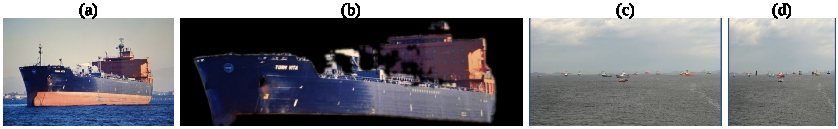
\includegraphics[width=0.8\textwidth]{figs/fig_composition_process.pdf}
  \caption{In-place synthetic composition pipeline. (a)~InaTechShips source. (b)~SAM-segmented crop. (c)~CITRA-3D-Real operational scene. (d)~Synthetic result after in-place substitution.}
  \label{fig:composition_process}
\end{figure*}

\subsection{CITRA-3D-Real: operational maritime dataset}\label{sec:citra3d}

The CITRA-3D-Real dataset was collected under a maritime surveillance programme coordinated by CASNAV (Centre for Naval Systems Analysis), using fixed coastal surveillance cameras positioned at elevated vantage points overlooking a bay area. Images have a native resolution of 1920$\times$1080 pixels and capture a variety of maritime conditions including clear skies, overcast weather, haze, and varying sea states. The dataset spans multiple months, providing temporal diversity in lighting and weather conditions.

The dataset contains 2,081 images with 7,003 annotated bounding boxes across 9 original vessel categories, which were collapsed into a single ``vessel'' class due to incompatible taxonomies between datasets and severe class imbalance (the smallest category contains only 8 instances). Annotations were produced by a single trained operator using LabelImg, with subsequent quality review. The dataset is used exclusively for civilian maritime surveillance research; no tactical, classified, or military operational parameters are disclosed. Institutional restrictions prevent disclosure of exact camera specifications and coordinates.

Table~\ref{tab:citra3d_profile} summarises the scale profile of the dataset. Following the COCO convention, objects with area smaller than $32 \times 32$ pixels after resizing to the 640-pixel evaluation resolution are considered small. The predominance of small objects (71.6\%) and the high object density (median 2, maximum 40 per image) characterise a challenging detection scenario. Vessels in CITRA-3D-Real occupy a median bounding-box area of only 0.10\% of the image, compared with 54\% in InaTechShips---a difference of approximately 500$\times$. Fig.~\ref{fig:scale_dist} contrasts these distributions.

\begin{table}[!htbp]
\caption{Scale profile of CITRA-3D-Real bounding boxes (normalised coordinates, 7,003 annotations).}\label{tab:citra3d_profile}
\begin{adjustbox}{max width=\columnwidth}
\begin{tabular}{@{}lcccccc@{}}
\toprule
Metric & Mean & Median & P10 & P90 & Min & Max \\
\midrule
Width  & 0.047 & 0.031 & 0.011 & 0.102 & 0.004 & 0.551 \\
Height & 0.046 & 0.032 & 0.013 & 0.096 & 0.004 & 0.438 \\
Area   & 0.004 & 0.001 & 0.0002 & 0.008 & 0.00003 & 0.211 \\
Objects/img & 3.37 & 2.0 & 1.0 & 7.0 & 1 & 40 \\
\bottomrule
\end{tabular}
\end{adjustbox}
\end{table}

The dataset is split into training (1,348 images, 4,489 boxes), validation (332 images, 1,267 boxes), and test (401 images, 1,247 boxes) sets.

\begin{figure*}[H]
  \centering
  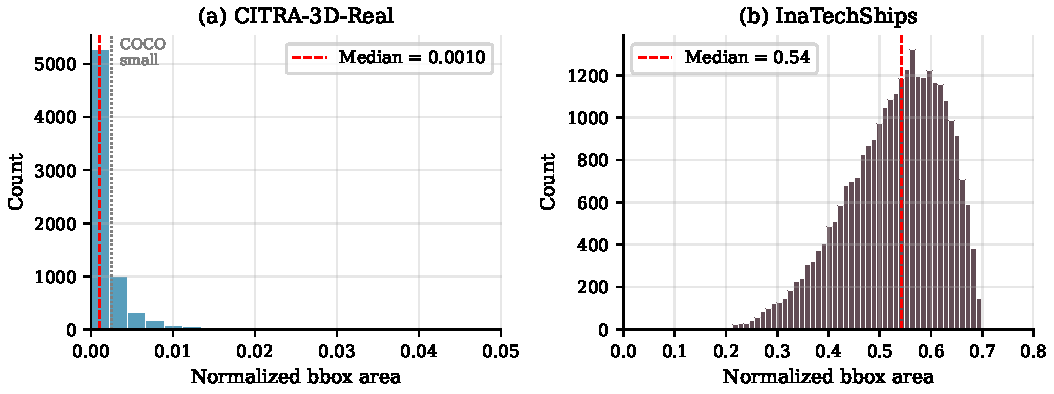
\includegraphics[width=0.8\textwidth]{figs/fig3_scale_distribution.pdf}
  \caption{Distribution of normalised bounding-box areas. (a)~CITRA-3D-Real (median 0.10\%). (b)~InaTechShips (median 54\%).}
  \label{fig:scale_dist}
\end{figure*}

\subsection{InaTechShips: public ship image dataset}\label{sec:inatechships}

The InaTechShips dataset \citep{teixeira2025inatechships} is sourced from shipspotting.com, a community of maritime photography enthusiasts. Images are professional-quality photographs of individual vessels, typically captured from close range at ports and harbours. Ships occupy a large portion of the image ($\sim$60--80\%), with one object per image and controlled lighting conditions.

Two subsets are used in this work:

\begin{itemize}
    \item \textbf{dataset\_25k\_v2 (curated):} 27,796 images selected via CLIP ViT-B-32 cosine similarity $\geq$ 0.60 against CITRA-3D-Real embeddings. Split 60/20/20 with disjoint partitions.
    \item \textbf{random\_pool\_v2 (random control):} 27,964 images randomly sampled from the same source with stratified downsampling to match the temporal distribution of the curated subset.
\end{itemize}

Labels for both subsets were generated using PointRend \citep{kirillov2020pointrend} by the original InaTechShips authors, ensuring methodological symmetry.

\subsection{Detector and hyperparameters}\label{sec:detector}

All experiments use YOLOv11m \citep{jocher2023ultralytics} with single-class detection. Hyperparameters were validated through formal HPO using Optuna TPE \citep{akiba2019optuna} with 30 trials across 5 dimensions (learning rate, optimiser momentum, weight decay, warmup epochs, learning rate schedule). The best configuration found was within 1$\sigma$ of the baseline ($\Delta$mAP50 = $-$0.0023), leading to the decision to retain the baseline configuration: AdamW optimiser, $lr_0 = 0.001$, $lr_f = 0.01$, cosine learning rate schedule, momentum 0.937, weight decay 0.0005, 3 warmup epochs, image size 640, batch size 16.

\subsection{Evaluation protocol}\label{sec:protocol}

Most sequential arms follow a two-stage protocol: (1) pre-training on the source dataset for 100 epochs with patience 20, and (2) fine-tuning on CITRA-3D-Real for 300 epochs with patience 30. The joint balanced arm follows a single-stage protocol in which real and synthetic samples are presented together, with real images repeated 13$\times$ to balance the 13 synthetic variations, during 300 epochs of training with patience 30; this yields 35,048 images per epoch (17,524 real + 17,524 synthetic). Table~\ref{tab:protocol} summarises the data pipeline and training regime for each arm. Evaluation is performed on the CITRA-3D-Real test set using mAP50 and mAP50-95 as primary metrics. Precision, Recall, and F1 are computed at IoU~=~0.5; the confidence threshold is selected on the validation set by the Ultralytics routine and applied unchanged to the held-out test set. No model selection was performed on the test set. Experiments are repeated with three seeds (42, 123, 2024) and results are reported as mean $\pm$ standard deviation.

\begin{table*}[!htbp]
\caption{Experimental protocol for each arm. Early stopping uses the corresponding validation partition: InaTechShips val during pre-training on A/B; synthetic val during pre-training on A' seq/frozen; CITRA-3D-Real val during all fine-tuning phases and for B1/B2/B2-long/A' joint.}\label{tab:protocol}
\begin{tabular}{@{}llclclc@{}}
\toprule
Arm & Init weights & Pre-train data & Epochs & Fine-tune data & Epochs & Seeds \\
\midrule
B1 & Random & --- & --- & CITRA-3D-Real & 300 & 3 \\
B2 & COCO & --- & --- & CITRA-3D-Real & 300 & 3 \\
B2-long & COCO & --- & --- & CITRA-3D-Real ($\times$13) & 300 & 1 \\
A  & COCO & InaTechShips curated & 100 & CITRA-3D-Real & 300 & 3 \\
B  & COCO & InaTechShips random  & 100 & CITRA-3D-Real & 300 & 3 \\
A' seq. & COCO & Synthetic (in-place) & 100 & CITRA-3D-Real & 300 & 3 \\
A' frozen & COCO & Synthetic (freeze=22) & 100 & CITRA-3D-Real & 300 & 3 \\
A' joint & COCO & --- & --- & CITRA-3D-Real + Synthetic (50/50) & 300 & 3 \\
A' joint-rand & COCO & --- & --- & CITRA-3D-Real + Synthetic random (50/50) & 300 & 3 \\
\bottomrule
\end{tabular}
\end{table*}

% ================================================================
% 4. METHOD: IN-PLACE SYNTHETIC COMPOSITION
% ================================================================
\section{Method: In-Place Synthetic Composition}\label{sec:method}

\subsection{Motivation}\label{sec:motivation}

As detailed in Section~\ref{sec:negative_transfer}, direct pre-training on InaTechShips images causes negative transfer due to a structural domain gap. Rather than discarding the public data, we propose adapting it to match the operational domain through synthetic image composition.

The key insight is that the domain gap manifests primarily in \emph{how} ships appear in the image (scale, position, context), not in \emph{what} ships look like (hull shape, superstructure). By extracting ship appearances from InaTechShips and placing them into the spatial context of CITRA-3D-Real, we can leverage the vessel diversity of the public dataset while respecting the operational characteristics of the target domain.

\subsection{Pipeline overview}\label{sec:pipeline}

The synthetic generation pipeline consists of four steps, illustrated visually in Fig.~\ref{fig:composition_process}:

\subsubsection{Step 1: Ship crop extraction with SAM}

For each image in the curated InaTechShips subset, we use the Segment Anything Model (SAM) \citep{kirillov2023segment} with the ViT-B backbone (checkpoint \texttt{sam\_vit\_b\_01ec64}, official Meta implementation). Masks are generated using the InaTechShips bounding box as prompt; the largest connected component is retained. The resulting crop is saved as an RGBA image with transparent background, enabling seamless compositing. No manual correction is applied. SAM is used here as part of the experimental data-generation pipeline, not for cosmetic alteration of manuscript artwork. A quality filter retains crops with mask coverage between 25--95\% of the bounding box area, minimum dimension $\geq$ 50 pixels, and aspect ratio between 0.2--8.0, yielding 23,828 usable crops from 27,796 images (85.7\% yield).

\subsubsection{Step 2: In-place substitution}

For each CITRA-3D-Real image, we generate multiple variations by substituting each annotated vessel with a randomly selected crop from the filtered pool. The crop is resized to exactly match the dimensions of the original bounding box and composited using alpha blending. Crucially, the labels remain identical to the originals---the bounding box coordinates are inherited directly from the operational annotations.

This approach reduces three sources of error present in conventional copy-paste methods:
\begin{itemize}
    \item \textbf{Placement:} because synthetic crops are anchored to real vessel annotations, placements are constrained to empirically observed vessel locations, reducing the risk of implausible placement on land, buildings, or sky.
    \item \textbf{Scale:} vessel sizes match the empirical distribution of the operational dataset by construction.
    \item \textbf{Density:} the number of objects per image matches the operational distribution exactly.
\end{itemize}

Source crops are resized directly to the target bounding-box dimensions. This preserves the empirical target-domain scale distribution but may geometrically distort source vessels when the source and target aspect ratios differ substantially. At operational scales---where 71.6\% of vessels occupy less than 32$\times$32 pixels---the resized crop fully occludes the original vessel beneath it. For the 2.9\% of large objects, minor blending artefacts may occur at mask boundaries, but these did not measurably affect detection performance.

\subsubsection{Step 3: Dataset generation}

To prevent data leakage, the CITRA-3D-Real train/validation/test split was established before synthetic generation. Training and validation synthetic images were generated exclusively from their corresponding real partitions. No test image, annotation, background, or bounding-box position was used in any training, validation, tuning, or model-selection step. Final evaluation was conducted solely on the held-out real CITRA-3D-Real test set.

We generate 13 variations per CITRA-3D-Real training and validation image, each with different randomly selected crops, producing a synthetic dataset of 21,840 training and validation images with 74,824 annotated objects (mean 3.37 per image, matching the operational distribution). The value of 13 variations was chosen to produce a synthetic training set of approximately 17,500 images, comparable in size to the InaTechShips curated training partition, while preserving the original target-domain split proportions.

% ================================================================
% 5. EXPERIMENTS AND RESULTS
% ================================================================
\section{Experiments and Results}\label{sec:results}

\subsection{Baselines}\label{sec:baselines}

Table~\ref{tab:baselines} shows the baseline results. COCO pre-training (B2) provides a substantial improvement over random initialisation (B1): +4.3 pp in mAP50 and +6.6 pp in mAP50-95, with non-overlapping mean $\pm$ standard deviation ranges across the tested seeds.

\begin{table}[!htbp]
\caption{Baseline results on CITRA-3D-Real test set (mean $\pm$ std, 3 seeds).}\label{tab:baselines}
\begin{adjustbox}{max width=\columnwidth}
\begin{tabular}{@{}llcc@{}}
\toprule
Arm & Pre-training & mAP50 & mAP50-95 \\
\midrule
B1 & Random init & 0.8008 $\pm$ 0.0061 & 0.4742 $\pm$ 0.0006 \\
\textbf{B2} & \textbf{COCO} & \textbf{0.8351 $\pm$ 0.0020} & \textbf{0.5055 $\pm$ 0.0022} \\
\bottomrule
\end{tabular}
\end{adjustbox}
\end{table}

\subsection{Negative transfer from direct pre-training}\label{sec:negative_transfer}

Table~\ref{tab:negative_transfer} presents the central finding: pre-training on InaTechShips images \emph{hurts} detection performance regardless of curation strategy.

\begin{table*}[htbp]
\caption{Direct pre-training results (mean $\pm$ std, 3 seeds).}\label{tab:negative_transfer}
\begin{tabular}{@{}llccc@{}}
\toprule
Arm & Pre-training data & mAP50 & mAP50-95 & $\Delta$ vs B2 \\
\midrule
B2 & COCO (baseline) & 0.8351 $\pm$ 0.0020 & 0.5055 $\pm$ 0.0022 & ref \\
A & Curated (3 seeds) & 0.7936 $\pm$ 0.0049 & 0.4692 $\pm$ 0.0017 & $-$4.15\% \\
B & Random (3 seeds) & 0.7945 $\pm$ 0.0046 & 0.4728 $\pm$ 0.0045 & $-$4.06\% \\
\bottomrule
\end{tabular}
\end{table*}

The curated and random subsets perform equivalently (difference of 0.09 percentage points, within 1$\sigma$ of Arm A variance), confirming that the negative transfer is independent of the selection strategy and stems from structural domain incompatibility.

\subsection{Epoch ablation: pre-training duration analysis}\label{sec:ablation}

To distinguish between recoverable overfitting and fundamental incompatibility, we varied the number of pre-training epochs (Table~\ref{tab:ablation}, Fig.~\ref{fig:ablation}).

\begin{table}[htbp]
\caption{Pre-training duration vs.\ fine-tuning performance (seed 42).}\label{tab:ablation}
\begin{adjustbox}{max width=\columnwidth}
\begin{tabular}{@{}cccc@{}}
\toprule
Pre-training epochs & mAP50 & mAP50-95 & $\Delta$ mAP50 vs B2 \\
\midrule
0 (B2 baseline) & 0.8351 & 0.5055 & ref \\
10 & 0.8200 & 0.4999 & $-$1.51\% \\
20 & 0.8171 & 0.4960 & $-$1.80\% \\
50 & 0.8037 & 0.4731 & $-$3.14\% \\
100 (Arm A) & 0.8006 & 0.4680 & $-$3.45\% \\
\bottomrule
\end{tabular}
\end{adjustbox}
\end{table}

In the seed-42 diagnostic experiment, degradation was monotonic across the tested pre-training durations: each increment of pre-training worsened the final result. Even 10 epochs of exposure reduced mAP50 by 1.5~pp. At 100 epochs, performance converged to the random initialisation level (B1 = 0.8008), suggesting, in this diagnostic setting, that extended pre-training on InaTechShips may erase the benefit of COCO weights.

\begin{figure}[H]
  \centering
  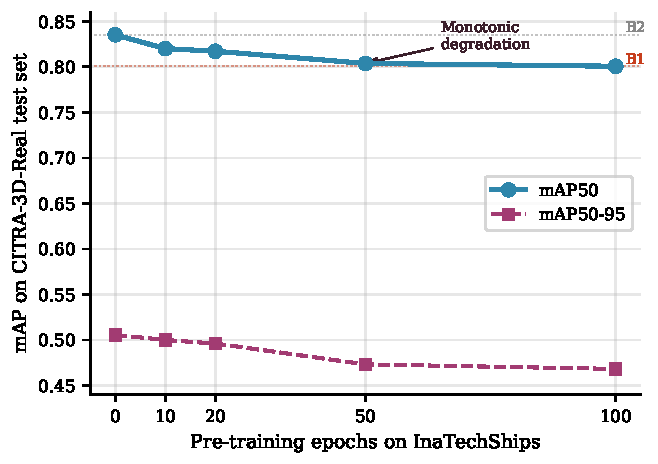
\includegraphics[width=\columnwidth]{figs/fig5_ablation_curve.pdf}
  \caption{Downstream detection performance vs.\ pre-training duration on InaTechShips (seed 42). Dashed lines: B2 and B1 reference levels.}
  \label{fig:ablation}
\end{figure}

\subsection{In-place synthetic composition results}\label{sec:synthetic_results}

We evaluated the in-place synthetic composition under three training regimes: sequential pre-training (100 epochs on synthetic, then 300 on real), frozen backbone pre-training (backbone frozen during synthetic phase), and joint balanced training (real and synthetic images combined in a single training run with 50/50 oversampling). Table~\ref{tab:main_results} and Fig.~\ref{fig:comparison} present the complete comparison.

\begin{table*}[htbp]
\caption{Complete results on CITRA-3D-Real test set, including the
      spatial-anchoring ablation (A' joint-rand) discussed in
      Section~\ref{sec:ablation_anchoring}. P, R and F1 at IoU = 0.5.
      \textsuperscript{$\dagger$}Single seed (42); volume-matched real-only control.}
\label{tab:main_results}
\begin{adjustbox}{max width=\textwidth}
\begin{tabular}{@{}llccccccc@{}}
\toprule
Arm & Pipeline & mAP50 & mAP50-95 & Precision & Recall & F1 & $\Delta$ mAP50 \\
\midrule
\textbf{A' joint} & \textbf{COCO $\rightarrow$ real+synth balanced (in-place)} & \textbf{0.8451 $\pm$ 0.0033} & \textbf{0.5206 $\pm$ 0.0017} & \textbf{0.857 $\pm$ 0.007} & \textbf{0.805 $\pm$ 0.003} & \textbf{0.830 $\pm$ 0.002} & \textbf{+1.00} \\
\textbf{A' joint-rand} & \textbf{COCO $\rightarrow$ real+synth balanced (random)} & \textbf{0.8457 $\pm$ 0.0058} & \textbf{0.5208 $\pm$ 0.0024} & \textbf{0.852 $\pm$ 0.009} & \textbf{0.804 $\pm$ 0.010} & \textbf{0.827 $\pm$ 0.005} & \textbf{+1.06} \\
B2 & COCO $\rightarrow$ CITRA-3D & 0.8351 $\pm$ 0.0020 & 0.5055 $\pm$ 0.0022 & 0.857 $\pm$ 0.005 & 0.783 $\pm$ 0.004 & 0.818 $\pm$ 0.002 & ref \\
B2-long & COCO $\rightarrow$ CITRA-3D $\times$13 & 0.8324\textsuperscript{$\dagger$} & 0.5107\textsuperscript{$\dagger$} & --- & --- & --- & $-$0.27 \\
A' frozen & COCO $\rightarrow$ synth (freeze) $\rightarrow$ CITRA-3D & 0.8342 $\pm$ 0.0039 & 0.5074 $\pm$ 0.0035 & 0.855 $\pm$ 0.001 & 0.774 $\pm$ 0.009 & 0.812 $\pm$ 0.005 & $-$0.09 \\
A' seq. & COCO $\rightarrow$ synth (100ep) $\rightarrow$ CITRA-3D & 0.8221 $\pm$ 0.0085 & 0.4933 $\pm$ 0.0059 & 0.828 $\pm$ 0.018 & 0.769 $\pm$ 0.010 & 0.797 $\pm$ 0.013 & $-$1.31 \\
B1 & Random $\rightarrow$ CITRA-3D & 0.8008 $\pm$ 0.0061 & 0.4742 $\pm$ 0.0006 & 0.829 $\pm$ 0.003 & 0.750 $\pm$ 0.002 & 0.787 $\pm$ 0.000 & $-$3.43 \\
B  & COCO $\rightarrow$ random pool $\rightarrow$ CITRA-3D & 0.7945 $\pm$ 0.0046 & 0.4728 $\pm$ 0.0045 & 0.856 $\pm$ 0.003 & 0.734 $\pm$ 0.014 & 0.790 $\pm$ 0.009 & $-$4.06 \\
A  & COCO $\rightarrow$ InaTechShips $\rightarrow$ CITRA-3D & 0.7936 $\pm$ 0.0049 & 0.4692 $\pm$ 0.0017 & 0.834 $\pm$ 0.008 & 0.735 $\pm$ 0.013 & 0.781 $\pm$ 0.004 & $-$4.15 \\
\bottomrule
\end{tabular}
\end{adjustbox}
\end{table*}

The joint balanced training (A' joint) achieves mAP50 = 0.8451 $\pm$ 0.0033, surpassing the COCO baseline (B2) by +1.00 percentage point. The mean $\pm$ standard deviation ranges do not overlap: A' joint $\in$ [0.8418, 0.8484] vs.\ B2 $\in$ [0.8331, 0.8371]; however, given the small number of seeds, this should be interpreted as preliminary evidence of a consistent improvement. The improvement in mAP50-95 is also notable (+3.0\% relative, 0.5206 vs.\ 0.5055). Importantly, Recall increases from 0.783 to 0.805 (+2.2~pp; +2.8\% relative), indicating that the model detects more vessels while maintaining Precision (0.857 vs.\ 0.857), yielding the highest F1 score (0.830) among all arms.

The training regime comparison reveals that the same synthetic data produces different outcomes depending on how it is used: sequential pre-training produces a forgetting-like degradation ($-$1.31~pp), frozen backbone largely neutralises the degradation ($-$0.09~pp, within the observed seed-level variability of B2), and joint balanced training appears to mitigate the forgetting-like degradation observed in the sequential regime while leveraging synthetic diversity (+1.00~pp).

To control for the effect of training volume, we ran a matched-steps experiment (B2-long): CITRA-3D-Real training images oversampled 13$\times$ (17,524 images, same gradient steps per epoch as A' joint) with no synthetic data. B2-long achieved mAP50 = 0.8324 in the seed-42 control, slightly below the standard B2 (0.8351), although its mAP50-95 was marginally higher (0.5107 vs.\ 0.5055). This suggests that repeated exposure to real images alone does not explain the A' joint improvement in mAP50, supporting the interpretation that increased training volume alone is unlikely to explain the A' joint mAP50 gain.

Table~\ref{tab:ap_size} presents AP and AR stratified by object size following COCO conventions (small: area $<$ $32 \times 32$ pixels; medium: $32 \times 32$ to $96 \times 96$; large: $> 96 \times 96$). The joint balanced arm shows mean improvements across all size categories, although the magnitude of these gains is modest. The most notable gain is in small-object recall (AR$_\text{small}$: 0.385 $\pm$ 0.007 $\rightarrow$ 0.400 $\pm$ 0.011, +0.015 absolute), which is operationally relevant given that 71.6\% of vessels in CITRA-3D-Real fall in this category. Sequential pre-training, by contrast, shows no improvement for small objects and slight degradation for medium and large objects.

\begin{table}[htbp]
\caption{Mean $\pm$ std AP and AR by object size across 3 seeds (COCO conventions).}\label{tab:ap_size}
\begin{adjustbox}{max width=\columnwidth}
\begin{tabular}{@{}lccc@{}}
\toprule
Metric & B2 & A' joint & A' seq. \\
\midrule
AP$_\text{small}$  & 0.255 $\pm$ 0.002 & \textbf{0.262 $\pm$ 0.011} & 0.255 $\pm$ 0.016 \\
AP$_\text{medium}$ & 0.571 $\pm$ 0.002 & \textbf{0.576 $\pm$ 0.008} & 0.565 $\pm$ 0.009 \\
AP$_\text{large}$  & 0.679 $\pm$ 0.001 & \textbf{0.691 $\pm$ 0.010} & 0.672 $\pm$ 0.012 \\
\midrule
AR$_\text{small}$  & 0.385 $\pm$ 0.007 & \textbf{0.400 $\pm$ 0.011} & 0.396 $\pm$ 0.011 \\
AR$_\text{medium}$ & 0.647 $\pm$ 0.004 & \textbf{0.655 $\pm$ 0.004} & 0.644 $\pm$ 0.004 \\
AR$_\text{large}$  & 0.751 $\pm$ 0.003 & \textbf{0.759 $\pm$ 0.010} & 0.745 $\pm$ 0.006 \\
\bottomrule
\end{tabular}
\end{adjustbox}
\end{table}

\begin{figure*}[H]
  \centering
  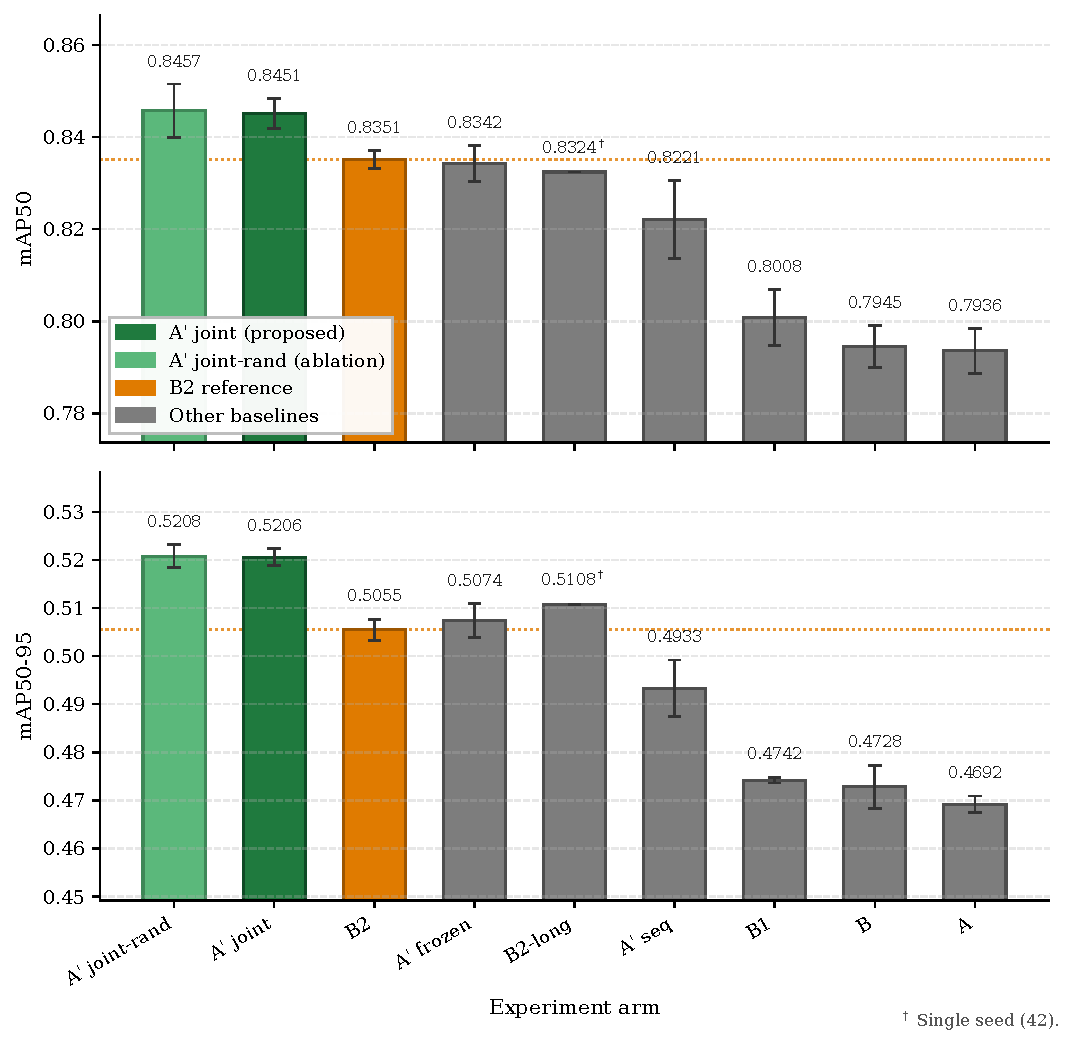
\includegraphics[width=\textwidth]{figs/fig6_comparison_bar_dual.pdf}
  \caption{mAP50 and mAP50-95 for all experimental arms on CITRA-3D-Real test set. Error bars indicate $\pm$1 standard deviation across three seeds. B2-long was run only with seed 42 and is shown without an error bar.}
  \label{fig:comparison}
\end{figure*}

\subsection{Ablation of spatial anchoring}\label{sec:ablation_anchoring}

A central design choice of our in-place composition pipeline is that synthetic vessels are placed at the exact positions of annotated real vessels in operational scenes. The rationale, as discussed in Section~\ref{sec:method}, is twofold: it produces visually plausible images (vessels are placed in sea regions where ships are expected to appear) and it preserves the spatial distribution of the operational domain. However, since both effects --- visual plausibility and spatial distribution preservation --- co-occur in the in-place design, the relative contribution of anchoring \emph{per se} to detection performance is not directly observable from the main comparison. To isolate this contribution, we evaluated an additional arm, A' joint-rand, in which the only difference from A' joint is the placement of synthetic crops.

\paragraph{Setup} In A' joint-rand, synthetic crops are placed at uniformly sampled positions within an adaptive sea region, rather than at the positions of real annotated vessels. The sea region is defined by a horizon line set adaptively at the top of the highest real bounding box per image, with a floor at 35\% of the image height to guard against label outliers (e.g., distant vessels near the cloud line). Before synthetic placement, real objects are removed via Telea inpainting (radius = 3 px, padding = 2 px) (Telea, 2004) to avoid introducing contradictory label signal --- a step that is unnecessary in A' joint, where the synthetic crop occupies the same region by construction. Crop sizes are sampled from the empirical width--height distribution of real CITRA-3D-Real bounding boxes; all other aspects --- crop pool, 13$\times$ variations, training hyperparameters, oversampling, and the 50/50 balanced regime --- are held constant.

\paragraph{Results} Table~\ref{tab:main_results} shows that A' joint-rand achieves mAP50 = 0.8457 $\pm$ 0.0058 and mAP50-95 = 0.5208 $\pm$ 0.0024, both statistically indistinguishable from A' joint (mAP50 = 0.8451 $\pm$ 0.0033, mAP50-95 = 0.5206 $\pm$ 0.0017). The two methods are also equivalent in F1 within their respective standard deviations (0.827 $\pm$ 0.005 vs.\ 0.830 $\pm$ 0.002). Both methods surpass the COCO baseline (B2 = 0.8351 $\pm$ 0.0020) by approximately one percentage point in mAP50, with non-overlapping ranges.

\paragraph{Interpretation} This near-equivalence suggests that, within the joint balanced training regime, the model is robust to the specific placement of synthetic objects, provided that placement remains within the sea region of the operational scene. The performance gain over B2 is therefore attributable to (i) crop visual diversity from InaTechShips, (ii) scale and density alignment with the operational domain, and (iii) the joint balanced training regime itself --- rather than to spatial anchoring at the exact positions of real objects. A small but consistent advantage of A' joint over A' joint-rand is observed in Precision and F1, suggesting that in-place anchoring may contribute marginally to localisation precision rather than to detection per se. We treat this as preliminary evidence given the small number of seeds and recommend further validation in future work.

\paragraph{Implication for the method} The in-place anchoring strategy remains the recommended default because it acts as a robust form of data sanitisation: it guarantees, by construction, that synthetic objects fall in plausible locations of the operational scene, eliminating the need for the inpainting step and the heuristics required to define an adaptive sea region. However, our results indicate that the core methodological contribution of this work --- the combination of domain-adapted synthetic composition with joint balanced training --- does not depend critically on this specific placement choice.

\FloatBarrier
% ================================================================
% 6. DISCUSSION
% ================================================================

\section{Discussion}\label{sec:discussion}

\subsection{Why direct transfer fails}

The negative transfer observed in Arms A and B is consistent with catastrophic forgetting or harmful intermediate feature adaptation \citep{mccloskey1989catastrophic, zhang2023negative}: the intermediate pre-training on InaTechShips may overwrite or de-emphasise generic low-level features learned from COCO (edges, textures, shapes) with domain-specific features optimised for close-range ship photography. These specialised features do not transfer to the operational domain, where ships appear as small, distant objects in complex maritime scenes. Notably, the generic COCO features---learned from 80 diverse object categories with no dedicated vessel class---appear more useful than 28,000 ship-specific images.

The ablation of spatial anchoring (Section~\ref{sec:ablation_anchoring}) further indicates that the gain is attributable to the combination of crop diversity, scale/density alignment, and the joint balanced training regime, rather than to the specific in-place placement of synthetic objects.

\subsection{Why in-place composition works}

The synthetic composition addresses all three axes of the domain gap simultaneously:

\begin{itemize}
    \item \textbf{Scale:} vessel crops are resized to match the operational distribution (median bounding-box area of 0.10\% of the image, compared with $\sim$54\% in InaTechShips). At this scale, fine-grained appearance differences between professional and operational photography become imperceptible.
    \item \textbf{Density:} multiple ships per image (mean 3.37) match the operational distribution, training the model to detect objects in cluttered scenes.
    \item \textbf{Context:} backgrounds are real operational scenes, providing authentic ocean surfaces, weather conditions, and coastal features.
\end{itemize}

\subsection{Why training regime matters}

A key finding is that the same synthetic data produces markedly different outcomes depending on the training regime. Sequential pre-training (COCO $\rightarrow$ synthetic $\rightarrow$ real) causes partial forgetting-like degradation: the model overwrites useful COCO features during the synthetic phase and cannot fully recover them during fine-tuning. Frozen backbone pre-training preserves COCO features but limits what the model can learn from synthetic data. Joint balanced training appears to mitigate this dilemma by presenting real and synthetic images simultaneously in each batch, encouraging the model to exploit synthetic diversity while remaining anchored to the real target-domain distribution.

The improvement in Recall (+2.2~pp, from 0.783 to 0.805) with maintained Precision (0.857) suggests that synthetic diversity helps the model recognise vessel appearances it would not encounter in the limited real training set alone. In maritime surveillance, missed detections (false negatives) are typically more costly than false alarms, making this Recall gain operationally relevant.

\subsection{CLIP similarity as a proxy for transferability}

The equivalence of Arms A and B (curated $\approx$ random, $\Delta$ = 0.09~pp) suggests that, in this setting, the tested global CLIP ViT-B-32 curation strategy did not capture the structural properties that determine transfer learning success. The three axes of incompatibility we identified---scale distribution, object density, and capture conditions---are not encoded in CLIP's embedding space, which operates at the holistic image level rather than at the object-detection level.

\subsection{Limitations}

Several limitations should be acknowledged. First, our evaluation uses a single operational dataset (CITRA-3D-Real) from one geographic location with specific camera configurations; generalisation to other maritime surveillance systems remains to be validated. Second, all experiments use a single detector architecture (YOLOv11m); the extent to which our findings transfer to other detectors such as RT-DETR or Faster R-CNN is unknown, though the domain gap analysis is architecture-independent. Third, while the synthetic images are visually convincing at operational scales (where vessels occupy a median area of 0.10\% of the image), close inspection reveals compositing artefacts at crop boundaries---this is unlikely to affect detection training but may matter for tasks requiring pixel-level precision. Fourth, the method requires annotated bounding boxes in the target domain to serve as anchor positions for composition, limiting its applicability to fully unsupervised scenarios. Fifth, the crop resizing does not enforce aspect-ratio matching between source crop and target bounding box, which may introduce geometric distortion for objects with extreme proportions. Finally, we include a sea-aware random placement baseline (A' joint-rand, Section~\ref{sec:ablation_anchoring}) but do not evaluate fully unconstrained random placement, which would permit vessels on land, buildings, or sky. Such a baseline is expected to produce contradictory training signal and was not considered methodologically informative.

% ================================================================
% 7. CONCLUSION
% ================================================================

\section{Conclusion}\label{sec:conclusion}

This paper investigated under which training conditions public ship imagery can be leveraged to improve vessel detection in operational maritime surveillance scenarios. We showed that direct use of InaTechShips images as pre-training data causes negative transfer ($-$4.15 pp mAP50), attributed to a structural domain gap in scale, density, and capture conditions. This gap affects curated and random subsets equally, indicating that CLIP-based visual similarity alone appears insufficient as a proxy for transfer learning compatibility.

We proposed in-place synthetic composition as a domain adaptation strategy: vessel crops segmented with SAM from public ship images are placed at the exact positions and scales of real vessels in operational scenes. The results suggest that synthetic data adaptation and training regime jointly determine whether positive transfer is achieved. Sequential pre-training on synthetic data reduces but does not eliminate the negative transfer ($-$1.31~pp). However, joint balanced training---combining real and synthetic images in equal proportions within the same training run---improves mAP50 by +1.00~pp over the COCO baseline across the tested seeds, while increasing Recall from 0.783 to 0.805 (+2.2 pp) without loss of Precision.

A controlled ablation isolating the effect of spatial anchoring shows that sea-aware random placement of synthetic crops reaches statistically equivalent detection performance to in-place anchoring (mAP50 = 0.8457 $\pm$ 0.0058 vs. 0.8451 $\pm$ 0.0033). This indicates that, within the joint balanced regime, the performance gain over the COCO baseline is attributable to crop diversity, scale and density alignment, and the 
training regime itself --- rather than to the specific positioning of synthetic objects. In-place anchoring nonetheless remains the recommended default because it eliminates the need for inpainting and sea-region heuristics, acting as automatic data sanitisation.

Although evaluated on a single operational maritime dataset, the results suggest that structurally aligned synthetic composition combined with an appropriate training regime may be a promising strategy for domains in which public source data differ from target operational imagery in scale, density, and context.

Future work includes extending the approach to multi-class detection, testing with alternative detector architectures (RT-DETR, Faster R-CNN), investigating the optimal ratio of real to synthetic images in joint training, and combining in-place composition with complementary augmentation strategies such as mosaic, mixup, or weather simulation.

% ================================================================
% DECLARATIONS (Elsevier order)
% ================================================================
\section*{CRediT authorship contribution statement}

\textbf{Daniela L. Freire:} Conceptualisation, Methodology, Software, Formal analysis, Validation, Investigation, Visualisation, Writing -- Original Draft, Writing -- Review \& Editing.
\textbf{Eduardo H. Teixeira:} Data Curation, Resources, Methodology, Writing -- Review \& Editing.
\textbf{Leandro A. S. Moreira:} Supervision, Project Administration, Funding Acquisition, Writing -- Review \& Editing.

\section*{Declaration of competing interest}

The authors declare that they have no known competing financial interests or personal relationships that could have appeared to influence the work reported in this paper.

\section*{Funding}

This work was supported by the Brazilian Navy under the CASNAV/DMarSup project (Termo 66/2025). The funder provided access to the restricted CITRA-3D-Real dataset. The authors were responsible for the study design, experiments, analysis, interpretation of results, manuscript preparation, and decision to submit the article for publication.

\section*{Data and code availability}

All source code, experiment configurations, and analysis scripts are publicly available at \url{https://github.com/DanielaLFreire/maritime-synthetic-detection}. The repository includes 22 scripts organised in six stages (data preparation, dataset acquisition, analysis, synthetic generation, training, and figure generation), YAML configuration files for each experimental arm, per-seed result CSVs, and JSON reports from all pipeline outputs. The CITRA-3D-Real images and derived synthetic images cannot be publicly released because they contain restricted operational maritime surveillance imagery and location-sensitive visual information. Aggregated statistics, configuration files, and per-seed metrics are available in the public repository. The InaTechShips dataset is publicly accessible through the original authors' repository \citep{teixeira2025inatechships}.

\section*{Declaration of generative AI and AI-assisted technologies in the manuscript preparation process}

During the preparation of this work, the authors used Claude (Anthropic) for assistance with code development, data analysis pipeline design, and manuscript organisation. No restricted images or confidential data were uploaded to generative AI tools. The authors reviewed and edited all AI-generated outputs and take full responsibility for the content of the publication.

\section*{Acknowledgements}

We thank CASNAV for providing the CITRA-3D-Real dataset and Eduardo H. Teixeira for sharing the complete PointRend label set for InaTechShips. Computational resources were provided by Google Colab Pro+ (NVIDIA A100 GPU).

% ================================================================
% REFERENCES
% ================================================================
%\clearpage
\bibliographystyle{cas-model2-names}
\bibliography{references}

\end{document}
